% Chapter X

\chapter{Assembling of a new Heat Flux Partitioning Model} % Chapter title

\label{ch:NewHFP} % For referencing the chapter elsewhere, use \autoref{ch:name} 

%----------------------------------------------------------------------------------------

\section{New model}


\section{General description of the model}
\label{sec:model}

The main goal of such a model is to provide a way to compute the wall temperature $T_{w}$ resulting from the applied wall heat flux $\phi_{w}$, or the other way around.

\npar
In order to try to be as extensive as possible regarding the different heat transfer mechanisms at stake, the wall heat flux is supposed to be split between 4 different contributions (Figure \ref{fig:HFP}) :

\begin{itemize}
\item A convective heat flux towards the liquid phase, unaffected by the presence of bubbles on the heater surface : $\phi_{c,l}$
\item A boiling heat flux, representing the energy removed from the wall to grow a bubble up to its lift-off diameter : $\phi_{b}$
\item A quenching heat flux, accounting for transient heat transfer to the liquid phase when bubbles slide or lift-off from the wall : $\phi_{q}$
\item A convective heat flux towards the vapor phase, representing the heat transfer occurring through the dry areas of the surface beneath the bubbles : $\phi_{c,v}$
\end{itemize}


\begin{figure}[h!]
\centering
\fbox{

\begin{tikzpicture}[scale=3.0]

\coordinate (O) at (0,0);
\coordinate (A1) at (1,0);
\coordinate (A2) at (2,0);
\coordinate (A3) at (3,0);
\coordinate (A) at (4,0);


%Sections and wall
\draw (O) -- (A);
\draw ($(O)-(0,0.03)$) -- ($(A)-(0,0.03)$);
\foreach \i in {0,...,19}
{
\draw (\i*0.2,0) -- (\i*0.2+0.05,-0.03);
}



%\draw[dashed, gray!70!white] (A1) --++ (0,1);
%\draw[dashed, gray!70!white] (A2) --++ (0,1);
%\draw[dashed, gray!70!white] (A3) --++ (0,1);



%Flow arrows
\foreach \i in {1,...,12} 
{
\coordinate (Oloc) at ($(O)+(-0.1,\i/13)$);
\draw[->,>=latex, gray!50!blue] (Oloc)--++({ln(1+0.05*\i)},0);
}

\draw ($(Oloc) + ({ln(1+0.05*12)},0)$) node[below right]{${\overline{U_{L}}}$};


%Liquid heat flux

\coordinate (Ophi) at (0.4,0);

\draw[->,>=latex, thick, blue!70!gray] ($(Ophi)+(0,-0.1)$)--($(Ophi)+(0,+0.1)$);
\draw ($(Ophi)+(0,-0.15)$) node{${\phi_{c,L}}$};


%Boiling heat flux
\coordinate (Ob) at (1.0,0);

\tikzmath{\alph = 40; \alphrad= \alph * pi / 180; \ray=0.15; \rayw = sin(\alphrad r) * \ray;}; %Geom values

\coordinate (Oarc) at ($(Ob)+({\ray * sin(\alphrad r)},0)$);
\shade[ball color = gray!40, opacity = 0.4] (Oarc) arc({-(pi/2-\alphrad) r}:{(pi+pi/2-\alphrad) r}:\ray);

\draw (Oarc) arc({-(pi/2-\alphrad) r}:{(pi+pi/2-\alphrad) r}:\ray);


\draw[->,>=latex, thick, brown!80!black] plot [smooth, tension=0.5] coordinates {($(Oarc)+(0,-0.1)$) ($(Oarc)+(0.05,+0.03)$) ($(Oarc)+(-0.05,+0.1)$)};

\coordinate (Oarc2) at ($(Oarc) + (-2*\rayw,0)$);
\draw[->,>=latex, thick, brown!80!black] plot [smooth, tension=0.5] coordinates {($(Oarc2)+(0,-0.1)$) ($(Oarc2)+(-0.05,+0.03)$) ($(Oarc2)+(+0.05,+0.1)$)};

\draw ($(Ob)+(0,-0.15)$) node{${\phi_{e}}$};



%Vapor convective flux
\coordinate (Ob) at (1.75,0);

\tikzmath{\alph = 40; \alphrad= \alph * pi / 180; \ray=0.2; \rw=\ray * sin(\alphrad r);};

\coordinate (Oarc) at ($(Ob)+(\rw,0)$);
\shade[ball color = gray!40, opacity = 0.4] (Oarc) arc({-(pi/2-\alphrad) r}:{(pi+pi/2-\alphrad) r}:\ray);

\draw (Oarc) arc({-(pi/2-\alphrad) r}:{(pi+pi/2-\alphrad) r}:\ray);

\draw[red, thick, densely dashed] (Oarc) --++ (-2*\rw, 0);

\draw[->,>=latex, thick, red!80!black] ($(Ob)+(0,-0.1)$)--($(Ob)+(0,+0.1)$);
\draw ($(Ob)+(0,-0.15)$) node{${\phi_{c,V}}$};



%Quenching heat flux
\coordinate (Ob2) at (2.75,0);

\tikzmath{\alph = 40; \alphrad= \alph * pi / 180;
\dalph=20; \dalphrad=\dalph*pi/180;
\alphadvrad=\alphrad - \dalphrad;
\alphrecrad=\alphrad + \dalphrad;
\ray=0.2; 
\rayadv=\ray *(1+cos(\alphrad r))/(1+ cos(\alphadvrad r);
\rayrec=\ray *(1+cos(\alphrad r))/(1+ cos(\alphrecrad r);};


\coordinate (Cb2) at ($(Ob2)+(0.03,{\ray * cos(\alphrad r)})$);
\draw[green!50!black,->, >=latex] (Cb2)--++({\ray+0.08},0); \draw ($(Cb2)+({\ray+0.08},0)$) node[above]{$\overline{U_{b}}$ }; %Bubble velocity


\coordinate (Oarc) at ($(Ob2)+({\ray * sin(\alphrad r)},0)$);

\shade[ball color = gray!40, opacity = 0.4] (Oarc) arc ({-(pi/2-(\alphadvrad)) r}:{(pi/2) r}:\rayadv) arc ({(pi/2) r}:{(pi+pi/2-(\alphrecrad)) r}:\rayrec);

\draw (Oarc) arc ({-(pi/2-(\alphadvrad)) r}:{(pi/2) r}:\rayadv) arc ({(pi/2) r}:{(pi+pi/2-(\alphrecrad)) r}:\rayrec);

\coordinate (Ob2) at (3.5,0.5);
\tikzmath{\ray=0.25;};

\shade[ball color = gray!40, opacity = 0.4] (Ob2) circle(\ray);
\draw (Ob2) circle(\ray);



\tikzmath{\rayspi=0.07;};

\draw[->,>=stealth,gray!50!blue] plot[domain=0:3.2,smooth,xshift=65,yshift=3] ({(\x *pi) r}:{\rayspi*(1-\x/6)}) ;
\draw[->,>=stealth,gray!50!blue] plot[domain=0:3.2,smooth,xshift=70,yshift=5] ({(\x *pi) r}:{\rayspi*(1-\x/6)}) ;

\coordinate (Ophisl) at ($(Oarc) - (\rayadv+\rayrec+0.05,0)$);
\draw[->,>=latex, thick, orange!90!gray] ($(Ophisl)+(0,-0.1)$)--($(Ophisl)+(0,+0.1)$);
\draw ($(Ophisl)+(0,-0.15)$) node{${\phi_{q,sl}}$};


\tikzmath{\rayspi=0.08;};

\draw[->,>=stealth,gray!50!blue] plot[domain=0:3.2,smooth,xshift=94,yshift=3] ({(\x *pi) r}:{\rayspi*(1-\x/6)}) ;
\draw[->,>=stealth,gray!50!blue] plot[domain=0:3.2,smooth,xshift=105,yshift=3] ({(\x *pi) r}:{\rayspi*(1-\x/6)}) ;


\coordinate (Ophiq) at ($(Ob2) - (0,0.5)$);
\draw[->,>=latex, thick, orange!90!gray] ($(Ophiq)+(0,-0.1)$)--($(Ophiq)+(0,+0.1)$);
\draw ($(Ophiq)+(0,-0.15)$) node{${\phi_{q,lo}}$};

\end{tikzpicture}

}
\caption{Sketch of the considered HFP  {\color{red} A terminer, je dois ajouter des flèches pour indiquer les flux !}}
\label{fig:HFP}Listing of the different physics parameter involved in bubble departure phenomenon 

\end{figure}


The supposed mechanisms yields the total wall heat flux partioning (\ref{eq:HFP}) :

\begin{align}
\label{eq:HFP}
\phi_{w}=\phi_{c,l} + \phi_{e} + \phi_{q} + \phi_{c,v}
\end{align}


In the following subsections, we focus out analysis on each term to detail its modeling.

\npar


\subsection{Convective heat fluxes}
\label{subsec:conv_HF}

The convective heat fluxes towards the liquid phase $\phi_{c,l}$ and the vapor phase $\phi_{c,v}$ can be written using an associated heat transfer coefficient (\ref{eq:conv_HF}) :

\begin{align}
\label{eq:conv_HF}
\phi_{c,l}=\orangemath{a_{c,l}} \bluemath{h_{c,l}}\parth{\redmath{T_{w}}-\bluemath{T_{l}}} ~\text{ and }~
\phi_{c,v}=\orangemath{a_{c,v}} \bluemath{ h_{c,v}}\parth{\redmath{T_{w}}-\bluemath{T_{v}}}
\end{align}



\subsection{Boiling heat flux}

The total energy associated with the nucleation of a bubble with a volume $V_{b}$ can be expressed as $V_{b}\rho_{v}h_{lv}$. If one knows the nucleation frequency $f$ at which bubbles are generated along with the nucleation site density on the heater surface $N_{sit}$, the resulting heat flux associated with the nucleation phenomenon can thus be written as (\ref{eq:boil_HF}) :

\begin{align}
\label{eq:boil_HF}
\phi_{b}&=\bluemath{N_{sit}} \bluemath{f} \orangemath{V_{b}} \rho_{v} h_{lv}
\end{align}

\subsection{Quenching heat flux}

The quenching heat flux accounts for the transient heat transfer which occurs when cold liquid is brought close to the wall when a bubble slides or lifts-off, thus disrupting the previously established thermal boundary layer.

\textsc{Del Valle} \& \textsc{Kenning} have supposed that this kind phenomenon can be represented as a semi-infinite transient heat transfer between the liquid at $T_{l}$ and the wall at $T_{w}$. Solving the conductive heat transfer problem yields an instantaneous heat flux expressed as Eq.~\ref{eq:inst_quench_HF}.

\begin{align}
\label{eq:inst_quench_HF}
\phi_{q}\parth{t} = \frac{\lambda_{l}\parth{\redmath{T_{w}}-\bluemath{T_{l}}} }{\sqrt{\pi \eta_{l} t} }
\end{align}


Therefore, we can average this heat flux over a time $t_{w}$, during which the quenching operates, and ponderating it both by the portion of the affected heater area $a_{q}$ and the fraction of quenching time over a total bubble nucleation cycle $t_{w}f$, yielding : 

\begin{align}
\phi_{q}&=\orangemath{a_{q}} \bluemath{t_{w}} \bluemath{f} \frac{1}{\bluemath{t_{w}} } \int_{0}^{  \bluemath{t_{w}} } \frac{\lambda_{l}\parth{\redmath{T_{w}}-\bluemath{T_{l}} }}{\sqrt{\pi \eta_{l} t }} = \orangemath{a_{q}} \bluemath{t_{w}} \bluemath{f} \frac{2 \lambda_{l} \parth{\redmath{T_{w}} - \bluemath{T_{l}} } }{\sqrt{\pi \eta_{l} \bluemath{t_{w}} } }
\end{align}


\subsection{Needed closure relationships}

After expressing each heat flux components of the global partitioning, the resulting formulations yields a first list of parameters for which closure relationships (or at least precise definition) are needed. Terms previously highlighted in \textcolor{orange}{orange} will be given a specific definition, terms in \textcolor{blue}{blue} require a closure law, wall temperature is indicated in \textcolor{red}{red}.

\npar

The different terms needing further development are listed below :

\begin{itemize}
\item The fractions of the heater area ponderating convective and quenching heat transfers : $a_{c,l}$, $a_{c,v}$ and $a_{q}$(\ref{sec:geometry})
\item The convective heat transfer coefficients : $h_{c,l}$ and $h_{c,v}$ (Section \ref{sec:HTC})
\item The nucleation site density over the heater surface : $N_{sit}$ (Section : \ref{sec:NSD})
\item The nucleation frequency, which includes both the growth time $t_{g}$ (Section \ref{sec:bubble_growth}) of a bubble and the waiting time $t_{w}$ ({\color{red} Je dois encore proposer une modélisation pour $t_{w}$, à discuter}) : $f=1/\parth{t_{g}+t_{w}}$
\item The total bubble volume $V_{b}$ (\ref{subsec:geom_bub}) generated until its lift-off, thus including the modeling of the bubble lift-off diameter : $D_{lo}$ 
\item The phases temperature : $T_{l}$ (\ref{subsec:liq_temp}) and $T_{v}$ (\ref{subsec:vap_temp})
\end{itemize}


\subsection{Single Bubble Quenching Area}

\begin{align}
A_{q,1b} = &
\begin{dcases}
\pi R_{lo}^{2} & \text{if } l_{sl}\leq R_{lo}-R_{d} \\
%
\frac{1}{2}\pi R_{d}^{2} + l_{sl}\parth{R_{d}+R_{lo}} + \frac{1}{2}\pi R_{lo}^{2} & \text{if } l_{sl} \geq R_{lo}+R_{d}
%
\end{dcases}
\end{align}

Which can be re-expressed by defining ${l_{sl}}^{*}=\dfrac{l_{sl}}{R_{lo}}$ and ${A_{q,1b}}^{*}=\dfrac{A_{q,1b}}{\pi R_{lo}^{2}}$

\begin{align}
{A_{q,1b}}^{*} = &
\begin{dcases}
1 & \text{if } {l_{sl}}^{*}\leq 1- \frac{R_{d}}{R_{lo}} \\
%
\frac{1}{2}\parth{1+\parth{\frac{R_{d}}{R_{lo}}}^{2} } + \frac{{l_{sl}}^{*}}{\pi}\parth{1+\frac{R_{d}}{R_{lo}}} & \text{if } {l_{sl}}^{*} \geq 1 + \frac{R_{d}}{R_{lo}}
\end{dcases}
\end{align}
and we linearly interpolate those two expressions for the region where $1-\dfrac{R_{d}}{R_{lo}}\geq {l_{sl}}^{*} \geq 1+\dfrac{R_{d}}{R_{lo}}$.


\subsection{Bubble Growth}


The question of the bubble growth law during its lifetime including sliding is still an open question that aims to cover various types of heat transfer mechanisms:

\begin{itemize}
\item Evaporation due to superheated liquid near the bubble base ;
\item Evaporation of a liquid microlayer trapped between the base of the bubble and the wall ;
\item Condensation on top of the bubble when it reaches subcooled liquid ;
\item Convective heat transfer due to relative velocity between the bubble and the liquid.
\end{itemize}

To our knowledge, many authors that have been tackling this issue had to consider empirical or fitted parameters when trying to exhaustively account for all the above heat transfers. For instance, Zhou \cite{zhou_experimental_2020} and Yoo \cite{yoo_development_2018} have proposed growth models that consider all the previously mentioned mechanisms. However, to fully close their mathematical model, many empirical values were used such as:

\begin{itemize}
\item The ratio between the bubble projected area and the microlayer area ;
\item The fraction of bubble area facing subcooling liquid ;
\item Value of coefficients in the condensation law \cite{levenspiel_collapse_1959}.
\end{itemize}

Moreover, those models postulate the existence of a microlayer contributing to the growth while recent numerical and experimental investigations showed that the bubble may as well grow with a microlayer or in a pure contact line regime depending on the operating conditions \cite{urbano_direct_2018, bures_modelling_2021, kossolapov_experimental_2021}.

In order to assess the force modeling proposed before, we choose a simpler growth law derived from heat conduction in the superheated liquid layer \cite{plesset_growth_1954}. 

\begin{equation}
R\parth{t} = K\Ja_{w} \sqrt{\eta_{L}t}
\end{equation}
where $K$ is an adjustable constant, with a value around the unity depending on the boiling conditions, often expressed as $K=\dfrac{2b}{\sqrt{\pi}}$.  In the case of pool boiling in an uniformly superheated liquid, Plesset \& Zwick \cite{plesset_growth_1954} found $b=\sqrt{3}$, Forster \& Zuber \cite{forster_growth_1954} obtained $b=\pi / 2$ while Zuber  \cite{zuber_dynamics_1961} stated that values of $b$ should be lying between 1 and $\sqrt{3}$. More recently, Yun \etal \cite{yun_prediction_2012} used $b=1.56$. We can thus observe that $K=2$ is likely to be an upper bound value for the growth constant. This value can thus be lower in the case of subcooled flow boiling. For instance, later comparisons with experimental measurements suggest values of $K$ slightly below 1 for subcooled flow boiling (Figure \ref{fig:slide_maity}).

This type of bubble growth has been widely used, and showed good agreement with many experimental observations and is particularly valid for early growth stages or small bubbles at high pressure \cite{kossolapov_experimental_2021, plesset_growth_1954, klausner_vapor_1993}.




\begin{table}[h!]

%\begin{changemargin}{-1cm}{0cm}

\noindent\makebox[\textwidth]{

\scriptsize
\centering
\begin{tabular}{p{20mm}|c c c c c c c c} 
Author & Fluid & $D_{h}$ [mm] & $P$ [bar] & $G_{L}$ [$\debm$] & $\Delta T_{L}$ [K] & $\phi_{w}$ [kW/m\up{2}] & $\Delta T_{w}$ [K] & $D_{d}$ [mm] ($N_{mes}$)\\
\hline
\\

Maity \cite{maity_effect_2000} \newline (2000) & Water & 20 & 1.01 & 0 - 239.6 & 0.3 - 0.7 & N.A. & 5 - 5.9 & 0.788 - 1.71 (9) \\

Kossolapov \cite{kossolapov} \newline (2021) & Water & 20 & 20 - 40 & 500 - 1500 & 0.3 - 0.7 & N.A. & 5 - 5.9 & 0.788 - 1.71 (9) \\

\hline
\end{tabular}
}


\caption{Bubble growth time data in vertical flow boiling}
\label{tab:tg_exp_data}

%\end{changemargin}

\end{table}

\subsection{Bubble Wait Time}

\begin{table}[h!]

%\begin{changemargin}{-1cm}{0cm}

\noindent\makebox[\textwidth]{

\scriptsize
\centering
\begin{tabular}{p{20mm}|c c c c c c c c} 
Author & Fluid & $D_{h}$ [mm] & $P$ [bar] & $G_{L}$ [$\debm$] & $\Delta T_{L}$ [K] & $\phi_{w}$ [kW/m\up{2}] & $\Delta T_{w}$ [K] & $D_{d}$ [mm] ($N_{mes}$)\\
\hline
\\

Maity \cite{maity_effect_2000} \newline (2000) & Water & 20 & 1.01 & 0 - 239.6 & 0.3 - 0.7 & N.A. & 5 - 5.9 & 0.788 - 1.71 (9) \\

\hline
\end{tabular}
}


\caption{Bubble wait time data in vertical flow boiling}
\label{tab:tw_exp_data}

%\end{changemargin}

\end{table}


\subsection{Nucleation Site Density}


\begin{table}[h!]

%\begin{changemargin}{-1cm}{0cm}

\noindent\makebox[\textwidth]{

\scriptsize
\centering
\begin{tabular}{p{20mm}|c c c c c c c c} 
Author & Fluid & $D_{h}$ [mm] & $P$ [bar] & $G_{L}$ [$\debm$] & $\Delta T_{L}$ [K] & $\phi_{w}$ [kW/m\up{2}] & $\Delta T_{w}$ [K] & $D_{d}$ [mm] ($N_{mes}$)\\
\hline
\\

Maity \cite{maity_effect_2000} \newline (2000) & Water & 20 & 1.01 & 0 - 239.6 & 0.3 - 0.7 & N.A. & 5 - 5.9 & 0.788 - 1.71 (9) \\

\hline
\end{tabular}
}


\caption{Nucleation Site Density data in vertical flow boiling}
\label{tab:nsit_exp_data}

%\end{changemargin}

\end{table}

The choice of a nucleation site density correlation can be a complicated matter since many different laws exist in the literature (Lemmert \& Chawla, Hibiki \& Ishii, Basu \etal, etc.).

\npar

In order to help us choosing an appropriate closure for $N_{sit}$, we compare 4 different correlations (Lemmert \& Chawla, Hibiki \& Ishii, Li \etal and Zhou \etal) to 4 different sets of experimental measurements of the NSD in various thermal-hydraulics conditions (Borishanskii \etal, Richenderfer \etal, Kossolapov, Zhou \etal). The results are presented on Figures 2.5 to 2.8 with error bars of $\pm 50 \%$.


\begin{figure}[h!]
\begin{multicols}{2}
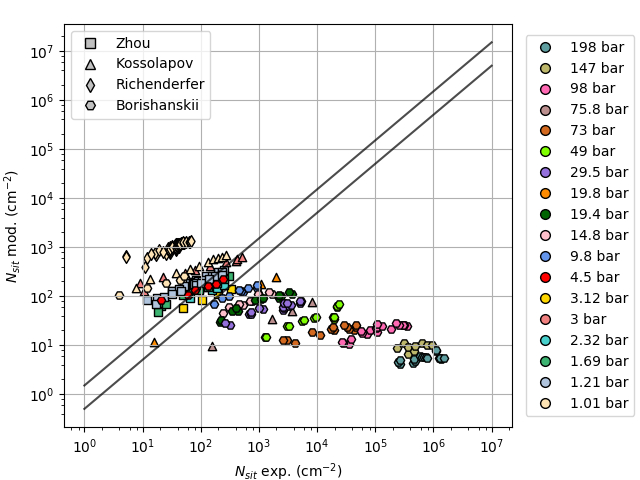
\includegraphics[width=1.0\linewidth]{img/NSD/LC.png}
\caption{Model from Lemmert \& Chawla}

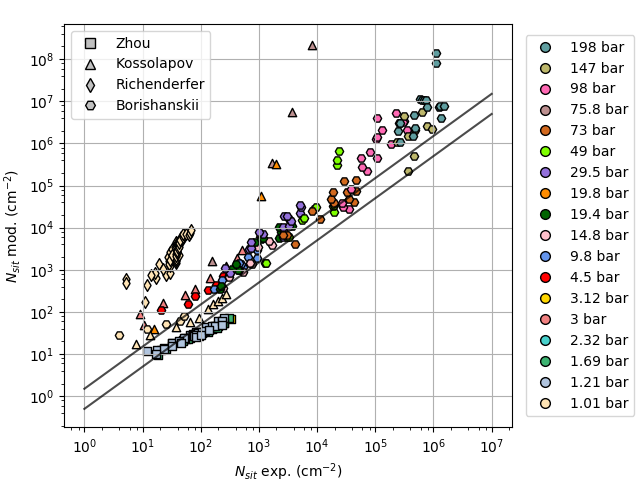
\includegraphics[width=1.0\linewidth]{img/NSD/HI_rtheta.png}
\caption{Model from Hibiki \& Ishii}
\end{multicols}
\end{figure}

\begin{figure}[h!]
\begin{multicols}{2}
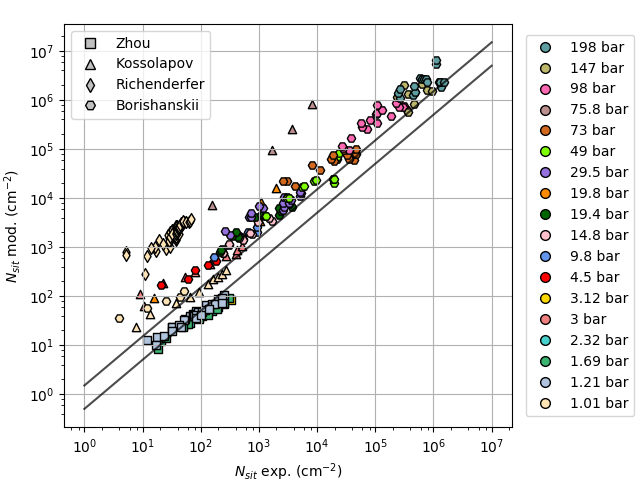
\includegraphics[width=1.0\linewidth]{img/NSD/Li_rtheta.png}
\caption{Model from Li \etal }

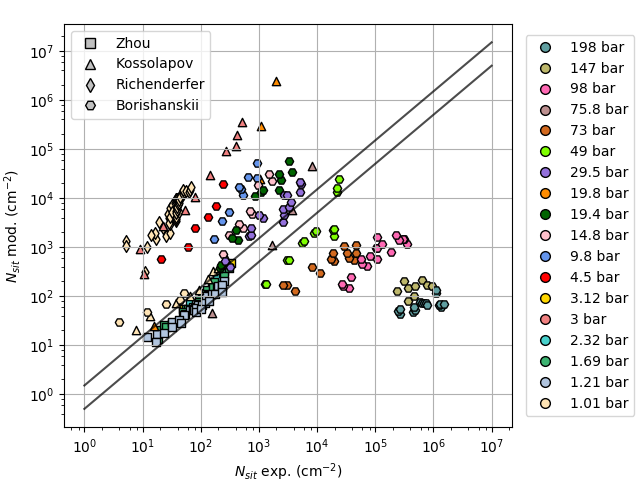
\includegraphics[width=1.0\linewidth]{img/NSD/Zhou_rtheta.png}
\caption{Model from Zhou \etal}
\end{multicols}
\end{figure}


As we can see, the model from Lemmert \& Chawla fails to correctly predict the nucleation site density at high pressures. Which is a direct consequence of its solely depedency on the wall superheat.

On the other hand, models such as those from Hibiki \& Ishii and Li \etal seem to better reproduce the different trends with flow conditions. 

Finally, altough the model of Zhou \etal includes a pressure term, its partial calibration on onyl low pressure data may explain the huge difference observed when trying to reproduce other experimental measurements.

{\color{red} Je vais ajouter un tableau des conditions TH de chacune des expériences + la formule détaillée de chacun des modèles.}

\subsection{Considerations on bubble interaction and nucleation sites deactivation}

NSD correlation actually compute the total number of sites where bubbles can nucleate on a surface. However, they do not represent how important a nucleation site will be in term of bubbles generation compared to another. 

\npar
In fact, Kossolapov has observed that each nucleation site has its own bubble nucleation frequency. Thus implying that some sites play a much greater role in wall nucleation compared to others. One can even consider that some nucleation sites can be neglected regarding their small impact on the whole phase change process.

\npar

In order to physically take into account this effect, Gilman considered a statistical approach, by assuming that nucleation site are randomly distributed over the heater surface (Complete Spatial Randomness). Then, considering that a nucleation site located under a bubble will be deactivated, one can express the number of sites actually contributing to bubble nucleation $N_{sit,a}$ as :


\begin{align}
N_{sit,a}=\parth{1-\mathcal{P}}N_{sit},\ \text{with}\ \mathcal{P}=1-e^{-N_{b}\pi \parth{D_{b}/2}^{2}}
\end{align}
where $N_{b}=t_{g}fN_{sit}$ is the actual average density of bubbles on the heater surface.

\npar

The resulting number of sites is a solution of the implicit equation on $N_{sit}$, which can be solved numerically or using the Lambert function (reciprocal of $w\rightarrow we^{-w}$).

\npar

{\color{red} Je vais détailler un peu plus cela avec des schémas clairs, ainsi qu'un exemple de comment cela pondère la densité de site totale, puisque cela permet d'éviter la divergence dans une loi telle que celle de Hibki \& Ishii à haute surchauffe pariétale} 



\subsection{Nucleation Sites and Bubbles Interactions}


\subsubsection{Static suppression}

If we suppose that the nucleation sites follow a homogeneous spatial Poisson process with an event density $\lambda$, we can express the probability of finding $n$ sites within an area A as :

\begin{align}
\mathcal{P}\parth{N\parth{A}=n}=\frac{\parth{\lambda A}^{n}}{n!}e^{-\lambda A}
\end{align}

If we consider the actual number of bubble-generating sites $N_{b}$, those sites are holding a bubble over a fraction $t_{g}f$ of the nucleation cycles in average. Thus, the actual density of bubbles held by the sites is : $t_{g}f N_{b}$. To derive $N_{b}$ from the value $N_{sit}$ provided by NSD correlations, we have to evaluate the probability of nucleation site overlapping, which corresponds to a distance $r$ lower than $R_{d}$ between two bubbles. 

\begin{align}
\mathcal{P}\parth{r\leq R_{d}} &=1-\mathcal{P}\parth{N\parth{\pi R_{d}^{2}}=0}\\
&=1-e^{-N_{b}t_{g}f\pi R_{d}^{2}} = \mathcal{P}
\end{align}

This probability thus represents the proportion of bubble that can't be geometrically accomodated on the surface. We can then evaluate $N_{b}$ from $N_ {sit}$ as :

\begin{align}
&N_{b}=\parth{1-\mathcal{P}}N_{sit} \\
%
\Leftrightarrow\  &N_{b}t_{g}f\pi R_{d}^{2}e^{N_{b}t_{g}f \pi R_{d}^{2}}= N_{sit}t_{g}f \pi R_{d}^{2} \\
%
\Leftrightarrow\   &N_{b} = \frac{\mathcal{W}\parth{N_{sit}\mathsf{A}}}{\mathsf{A}}\ \ \ \text{where}\ \ \ \mathsf{A}=t_{g}f\pi R_{d}^{2}
\end{align}



\subsubsection{Static coalescence}

Now that the actual number of bubble-generating sites have been identified, we can consider other interaction phenomena that can occur on the boiling surface. For instance, if two sites are simultaneously generating a bubble at a distance $d$ between $R_{d}$ and $2R_{d}$, the bubbles will coalesce while growing up to the detachment diameter. To estimate the probability of having a bubble on a site in this distance range, we consider the probability density function of the nearest-neighbour in the case of a homogeneous spatial Poisson process $f$ with an event density $\lambda$. 

\begin{align}
f\parth{r}=2\lambda \pi r e^{-\lambda \pi r^{2}}
\end{align} 

The considered probability of interaction is then :

\begin{align}
\mathcal{P}\parth{R_{d}\leq r \leq 2R_{d}} &=\int_{R_{d}}^{2R_{d}}f\parth{r} \mathrm{d}r \\
%
&= e^{-\lambda \pi R_{d}^{2}} - e^{-4\lambda \pi R_{d}^{2}}\\
%
&= e^{-\lambda \pi R_{d}^{2}}\crocht{1-\parth{e^{-\lambda \pi R_{d}^{2}}}^{3}} \\
&= \mathcal{P}_{coal,st} \ \ \ \text{with}\ \ \ \lambda=t_{g} f N_{b}
\end{align}

The density of bubble-generating sites that will lead to a static coalescence can then be estimated as :

\begin{align}
N_{coal,st}=\mathcal{P}_{coal,st}N_{b}
\end{align}

If we suppose that coalescing bubbles will instantly lift-off due to the perturbation associated with the coalescence process, this yields an associated boiling flux :

\begin{align}
\phi_{e,coal,st}=N_{coal,st} f \rho_{V}h_{LV} \frac{4}{3}\pi R_{coal,st}^{3} \ \ \ \text{where}\ \ \ R_{coal,st}=\sqrt[3]{2}R_{d} 
\end{align}

considering that the bubbles will merge approximately at $R=R_{d}$.

\subsubsection{Sliding coalescence}

Now that suppressed sites and sites that will lead to static coalescence have been identified, the remaining sites $N_{sl}=\parth{1-\mathcal{P}_{coal,st}}N_{b}$ will generate sliding bubbles. While sliding, a single bubble swipes an area :

\begin{align}
A_{sl, 1b} \approx l_{sl,1b}\frac{D_{d}+D_{lo}}{2}
\end{align}

In this area, there are an average number of bubble-generating sites $N_{b}A_{sl,1b}$ and an average number of growing bubbles on their sites $t_{g}f N_{b}A_{sl,1b}$

\npar
Two situations can happen from the sliding process :

\begin{itemize}
\item The bubble slides without coalescing
\item The bubble coalesces while sliding with a bubble growing on its site and lifts-off
\end{itemize}


Following the same approach from the static suppression, we can estimate the probability of finding no growing bubble over the sliding surface : 

\begin{align}
\mathcal{P}\parth{N\parth{A_{sl,1b}}=0 }=e^{-N_{b}t_{g}fA_{sl,1b}}
\end{align}

Thus, if a sliding bubble among the $N_{sl}$ does not encounter any growing bubble, the sites on its sliding area will be wiped and thus be quenched by cold liquid. This means that those sites will be suppressed due to the sliding of other bubbles over them.

Among the $N_{b}$ bubble generating sites we can identify 4 categories of sites :

\begin{itemize}
\item Sites generating bubbles which will slide without encountering any growing bubble on their path : $$N_{sl, NC}=N_{sl}e^{-ft_{g}N_{b}A_{sl,1b}}$$

\item Sites generating bubbles that will coalesce with a growing bubble during sliding : 
$$N_{sl, C}=  N_{sl}\parth{1-e^{-ft_{g}N_{b}A_{sl,1b}}}$$

\item Sites which will be suppressed by bubbles sliding without coalescing : $$N_{sup, sl}=N_{sl,NC}\ N_{b}A_{sl,1b}$$

\item Sites generating bubbles that will coalesce with a sliding bubble coming from upstream. Those bubbles are still in the growing phase up to detachment when they are coalescing with sliding bubbles. Therefore, there are equal to the number of sliding bubbles that will coalesce : $$N_{g,C}=N_{sl,C}$$

\end{itemize}

This allows to finally write :

\begin{align}
N_{b}&=N_{sl,NC}+N_{sl,C}+N_{sup,sl} + N_{g,C}\\
%
&=N_{sl}\crocht{2-e^{-ft_{g}N_{b}A_{sl,1b}}\parth{A_{sl,1b}N_{b}-1}}
\end{align}

Which finally yields the total number of sliding bubbles : 

\begin{align}
N_{sl}=\frac{N_{b}}{2-e^{-ft_{g}N_{b}A_{sl,1b}}\parth{A_{sl,1b}N_{b}-1}}
\end{align}